\documentclass[11pt,english]{article}
\usepackage{babel}
\usepackage[margin=1.3in]{geometry}
\usepackage{graphicx}
\usepackage{amsmath, amsfonts, amsthm, amssymb}
\usepackage{enumerate}
\usepackage{pdfpages}
\usepackage[toc,page]{appendix}
\usepackage{multicol}

%%%%%%%%%%%%%%%%%%%%%%%%HEADER%%%%%%%%%%%%%%%%%%%%%%%%%%%%%
\title{
{\normalsize \bf Technical Communication for Computer Scientists\\
Summer 2013}\\
\vspace{4cm}
{\bf Progress Report:\\The Movie-Chain-Runner Project}}
\author{
\\Team Chain-Runner \\\\
Sung Uk Ryu\\
Eugene Scanlon\\
Shashank Singh\\
Jimmy Zong
}
%%%%%%%%%%%%%%%%%%%%%%%%%%%%%%%%%%%%%%%%%%%%%%%%%%%%%%%%%%%

\begin{document}

\pagenumbering{gobble} % exclude page-numbering for title page and ToC
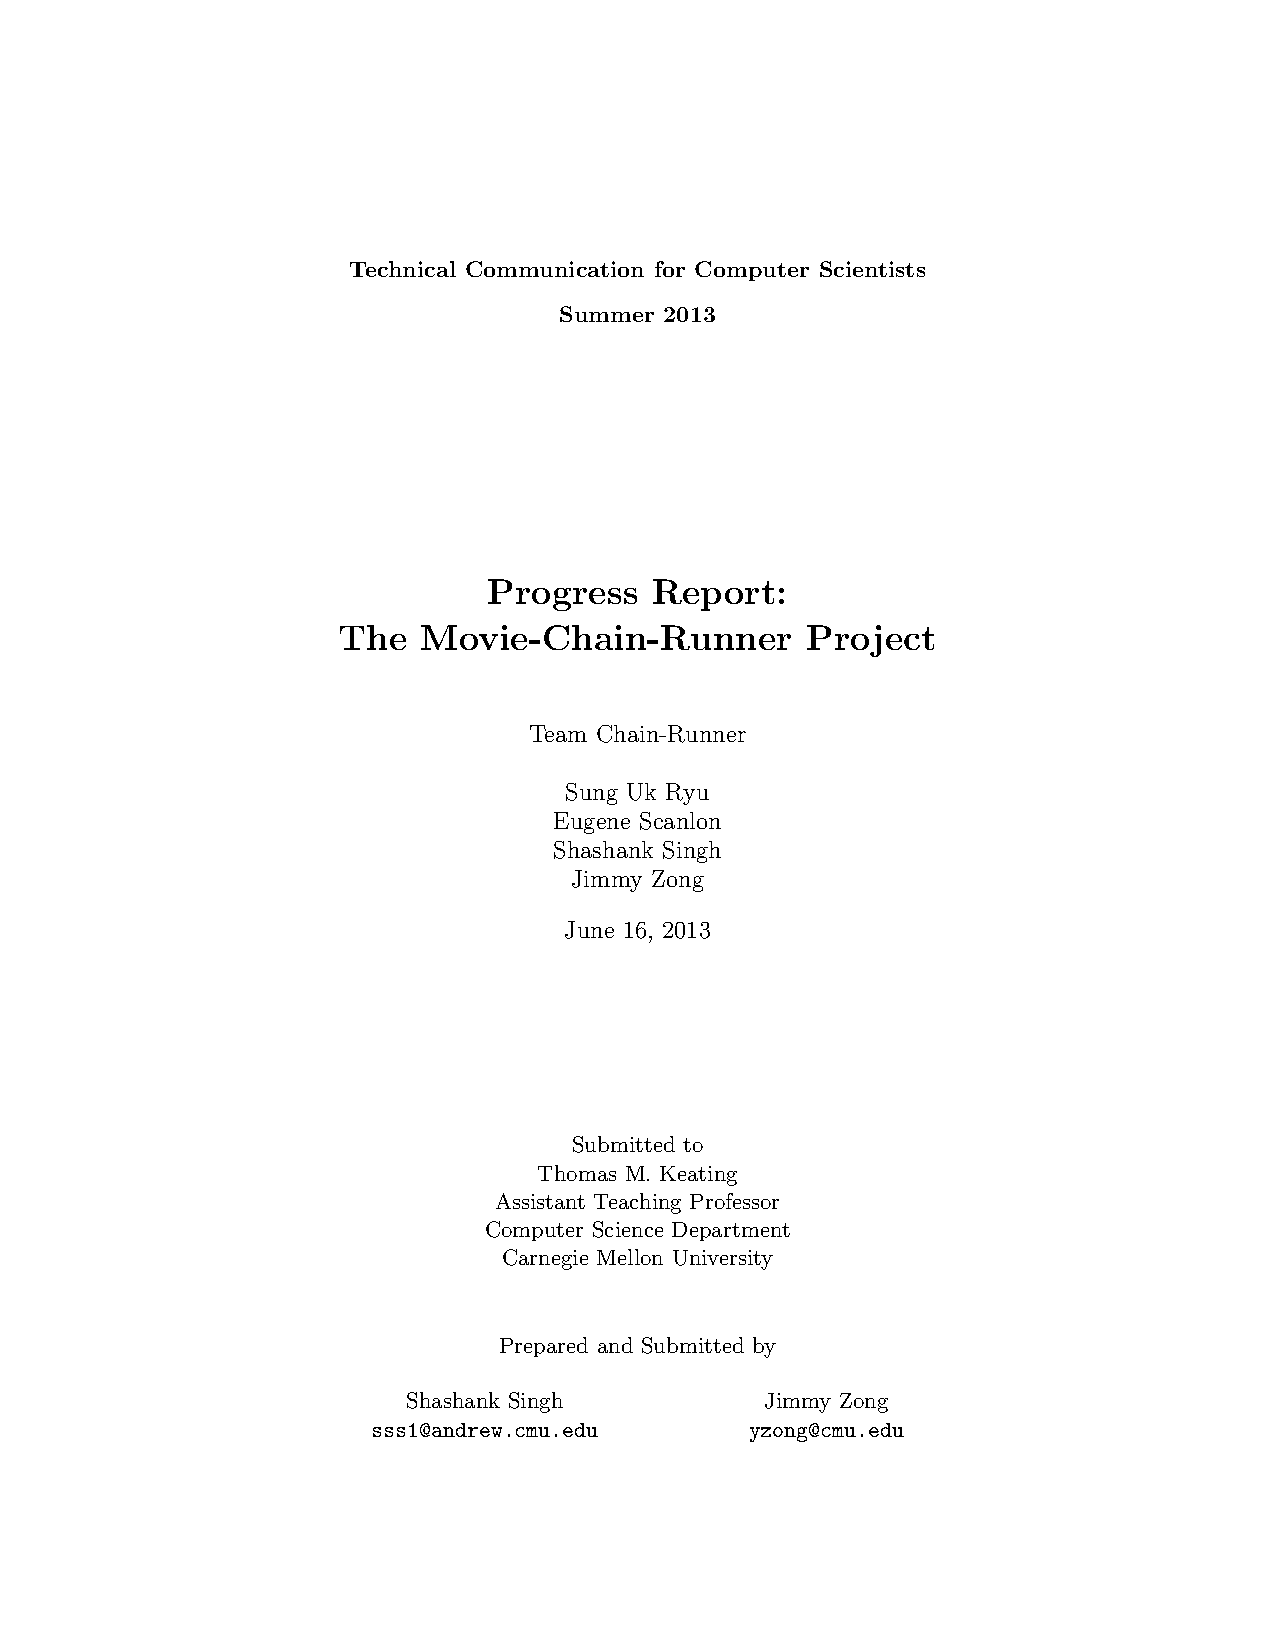
\includepdf{cover/cover.pdf}

\tableofcontents

\newpage
\pagenumbering{arabic} % include page-numbering starting here
\section{Overview}
We first explain the context of this report and the Movie-Chain-Runner Problem.
\subsection{This Report}
This report documents our progress in solving the Movie-Chain-Runner Problem
(discussed below) as of June 17, 2013, as well as our plans for how to proceed
up until the project deadline of June 27, 2013.

\subsection{The Movie-Chain-Runner Project}

\section{Progress}
We present our progress in three sections: General Progress, Status, and
Projections.

\subsection{General Progress}
Here we discuss the accomplishments of our project thus far.

Our first step was to reconstruct the list of movie titles as a directed graph,
with an edge from title $A$ to title $B$ when $B$ can follow $A$ in a movie
chain, reducing the problem to the well-known Longest Path Problem.
We proceeded to implement a greedy brute force algorithm which simply followed
as many paths as possible. This quickly constructed a path of 243 titles and
then ceased to make appreciable progress. The majority of our efforts have
since been towards honing and augmenting this brute force algorithm.

We have 

\subsection{Status}
Here we evaluate the current state of our project and discuss our ability to
meet deadlines set in our Proposal.

Our longest chain currently consists of ??? titles and ???? words. This falls
short of our scheduled June 17 goal of 285 titles and ???? words by ? titles
and ?? words.

Figure \ref{fig:gantto} on page ? shows the original Gantt chart presented in
our project proposal. We have made ?????????????? changes.
\begin{figure}[h]
\begin{center}
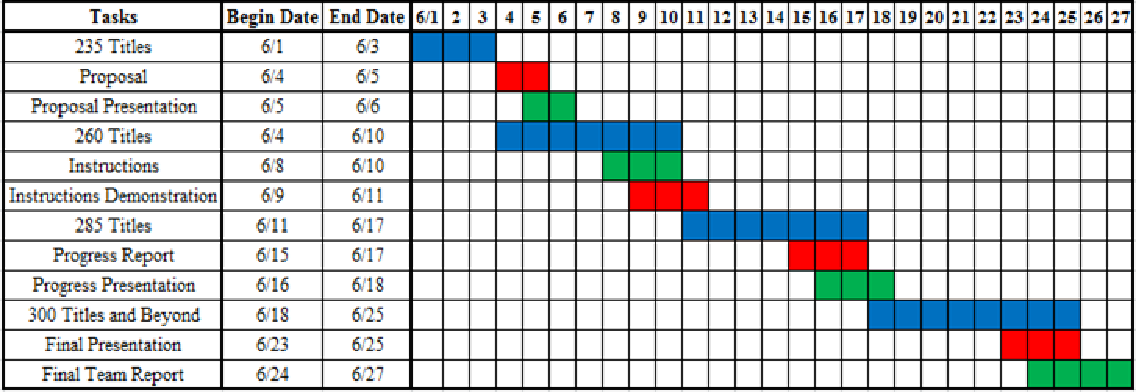
\includegraphics[width=\textwidth]{gantto}
\end{center}
\vspace{-0.5cm}
\caption{Our original Gantt chart.}
\label{fig:gantto}
\end{figure}

\subsection{Projections}
Here we discuss our goals from now until the final project deadline (June 27,
2013) and how we intend to accomplish these goals.

Since 285 titles and ???? words is the threshold for receiving A on this
project, the benefits of achieving 300 titles are primarily cosmetic. Thus, we
have reduced our final goal to 285 titles.

We have propose 3 approaches to this goal

Although we have devoted much computational power toward extending the longest
chain at either end, we have not considered a potentially large number
of alternative paths between nodes in the chain. Thus, we will attempt to
compute, for adjacent or nearby nodes, alternative (longer) chains connecting
the same nodes. We are also considering ways to ``trim'' the graph by removing
nodes unlikely to be in the longest chain, thus reducing the number of possible
paths that must be considered.

If simple methods prove insufficient, we may also implement a color-coding
algorithm proposed by Alon et al.
\footnote{Noga Alon , Raphael Yuster , Uri Zwick, Color-coding, Journal of the
ACM (JACM), v.42 n.4, p.844-856, July 1995. (accessed June 16, 2013 at
\texttt{http://dl.acm.org/citation.cfm?id=210337}).}
or one of several genetic algorithms proposed by Portugal et al.,
\footnote{
D. Portugal, C. H. Antunes, R. Rocha, ``A Study of Genetic Algorithms for
Approximating the Longest Path in Generic Graphs,'' Proc. of the IEEE SMC, pp.
2539-2544, 2010. (accessed June 16, 2013 at
\texttt{http://ieeexplore.ieee.org/xpl/articleDetails.jsp?arnumber=5641920\&
navigation=1}).}
although, due to the implementation complexity of these algorithms, we hope
this will be unnecessary.

\section{Recommendations}

\section{Discussion}

\begin{appendices}
\section{Our Longest Movie Chain}
Here, we include our current longest movie chain, with ??? titles and ????
words:
\begin{multicols}{3}
\begin{verbatim}
Die Another Day
Day of the Dead
Dead Poets' Society
Title 4
Title 5
Title 6
\end{verbatim}
\end{multicols}
\end{appendices}
\end{document}
